\section{Mise en place du projet}
\vspace{1cm}

Afin de répondre à ces objectifs, il m’a fallu mettre en place un plan d’action en prenant compte les technologies utilisées pour ce projet.\\
Mon travail devait pouvoir être maintenu facilement par mon tuteur, et pour ce faire la documentation et l’organisation des fichiers étaient primordiales.

\begin{commentaire}
    Une documentation complète a été réalisée en fin de projet pour apporter une précision supplémentaire aux commentaires écrits avec le standard d'écriture PHP Docs, permettant ainsi de faciliter la compréhension et la reprise du projet par mon tuteur.
\end{commentaire}

J'ai décidé de travailler en Programmation Orientée Objet (POO) pour faciliter la réutilisation des composants.\\
J’ai donc pensé à organiser mes fichiers par entité qui compose ce projet : chaque classe concernant une entité se trouve dans un dossier différent des autres et permet ainsi de facilement s’y retrouver dans les fichiers.

\begin{figure}[!h]
    \centering
    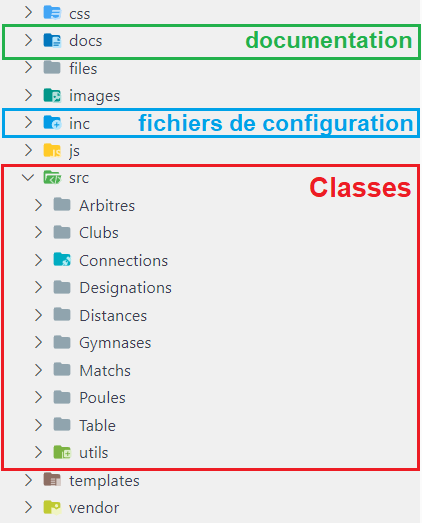
\includegraphics[width=0.5\linewidth]{architecture.png}
    \caption{Arborescence des dossiers du projet}
\end{figure}

\pagebreak

Pour effectuer cette séparation des fichiers sans compliquer l’utilisation des classes, j’ai adopté le concept de namespace et utilisé le gestionnaire de dépendances Composer pour ce projet.

\begin{commentaire}
    Composer est un gestionnaire de dépendances pour PHP. Il permet de réduire l’importation de fichiers en automatisant cette tâche.
\end{commentaire}

\vspace{2cm}

\faIcon{arrow-alt-circle-right} Je commencerai par expliquer les méthodes utilisées pour récupérer les données nécessaires à ce projet, puis j’exposerai les modifications apportées à l’interface graphique et enfin je parlerai en profondeur de l’algorithme d’automatisation des désignations.